\documentclass[a4paper, 10pt]{report}


\usepackage[utf8]{inputenc}
\usepackage{graphicx}
\usepackage{german}
\usepackage{mathtools}
\usepackage{setspace}
\usepackage{fancyhdr}
\usepackage{nameref}
\usepackage[hidelinks]{hyperref}
\usepackage{xcolor}
\usepackage[gen]{eurosym}
\usepackage{float}
\usepackage{mcode}
\setcounter{tocdepth}{3}
\setcounter{secnumdepth}{3}
\renewcommand{\chaptername}{}

\pagestyle{fancy}
\renewcommand{\headrulewidth}{0.4pt}
\renewcommand{\footrulewidth}{0.4pt}
\fancyhf{}
\lhead{{\footnotesize \textnormal{325.040}}}
\rhead{{\footnotesize \textnormal{Projekt 47}}}
\cfoot{{\footnotesize \textnormal{\thepage}}}
%\lfoot{{\footnotesize \textnormal{xxx}}}
%\rfoot{{\footnotesize \textnormal{\today}}}


\hypersetup{
    colorlinks,
    linkcolor={black},
    citecolor={blue!50!black},
    urlcolor={blue!80!black}
   }

\lstset{ %
  language=Matlab,                % the language of the code
  basicstyle=\small,              % the size of the fonts that are used for the code
  numbers=left,                   % where to put the line-numbers
  numberstyle=\tiny\color{gray},  % the style that is used for the line-numbers
  stepnumber=1,                   % the step between two line-numbers. If it's 1, each line 
                                  % will be numbered
  numbersep=5pt,                  % how far the line-numbers are from the code
  backgroundcolor=\color{white},      % choose the background color. You must add \usepackage{color}
  showspaces=false,               % show spaces adding particular underscores
  showstringspaces=false,         % underline spaces within strings
  showtabs=false,                 % show tabs within strings adding particular underscores
  frame=single,                   % adds a frame around the code
  rulecolor=\color{black},        % if not set, the frame-color may be changed on line-breaks within not-black text (e.g. commens (green here))
  tabsize=2,                      % sets default tabsize to 2 spaces
  captionpos=b,                   % sets the caption-position to bottom
  breaklines=true,                % sets automatic line breaking
  breakatwhitespace=false,        % sets if automatic breaks should only happen at whitespace
  title=\lstname,                   % show the filename of files included with \lstinputlisting;
                                  % also try caption instead of title
  keywordstyle=\color{blue},          % keyword style
  %commentstyle=\color{dkgreen},       % comment style
  %stringstyle=\color{mauve},         % string literal style
  escapeinside={\%*}{*)},            % if you want to add LaTeX within your code
  morekeywords={end,sortrows}               % if you want to add more keywords to the set
}




%----------------------------------------------------------------------------------------
%	TITLE PAGE
%----------------------------------------------------------------------------------------

\newcommand*{\titleGM}{\begingroup % Create the command for including the title page in the document
\hbox{ % Horizontal box
\hspace*{0.2\textwidth} % Whitespace to the left of the title page
\rule{1pt}{\textheight} % Vertical line
\hspace*{0.05\textwidth} % Whitespace between the vertical line and title page text
\parbox[b]{0.75\textwidth}{ % Paragraph box which restricts text to less than the width of the page

{\noindent\Huge\bfseries Kontinuierliche\\ Simulation}\\[2\baselineskip] % Title
{\large 325.040 - Projekt 47 - \textit{Sommersemester 2016}}\\[4\baselineskip] % Tagline or further description
{\textsc{Fabian Wedenik - 1426866 \newline
	Alexander Wimmer - 1328958 \newline
	Felix Hochwallner - 1328839 \newline
	Oskar Fürnhammer - 1329133}} % Author name
\\ \\ \\ \\


\vspace{0.5\textheight} % Whitespace between the title block and the publisher
{
\includegraphics[width=0.5cm]{TU-Logo}\noindent \ \ E325 Institut für Mechanik und Mechatronik}\\[\baselineskip] % Publisher and logo
}}
\endgroup}

%----------------------------------------------------------------------------------------
%	BLANK DOCUMENT
%----------------------------------------------------------------------------------------

\begin{document}
\thispagestyle{empty} % Removes page numbers
\titleGM % This command includes the title page
\newpage

\tableofcontents %inhaltsverzeichnis

\listoffigures %abbildungsverzeichnis



%---------------------------------------------------------------------------------------------------Vorwort------------------------------------------------------------------------------------------------
\renewcommand{\thechapter}{} %um ziffern vor überschriften im tableofcontents zu unterdrücken
\chapter{Vorwort}
\renewcommand{\thechapter}{1}
%
Sehr geehrte Damen und Herren, liebe Leser und Leserinnen!
\\
\\
Das vorliegende Protkoll wurde im Rahmen der Vorlesung und Übung \textit{Kontinuierliche Simluation (325.040/325.041)} verfasst und beschäftigt sich mit der Implementierung einer einfachen Regelung eines mechanischen Doppelpendels, sowohl in MATLAB, als auch in MalpeSim. \\
Dadurch soll unter anderem ein Vergleich zwischen klassischer textuelle Programmierung und grafischer, blockorientierter Modellierung gezogen werden. Betreut wurde das Projekt der Gruppe 47 von Fabian Germ.
\\
\\
Viel Spaß beim Lesen wünschen

%-----------------------------------------------------------------------------------------------------------------------------------------------------------------------------------------------------------
%												Chapter ****
%-----------------------------------------------------------------------------------------------------------------------------------------------------------------------------------------------------------
\renewcommand{\thechapter}{}
\chapter{Aufgabenstellung}
\renewcommand{\thechapter}{1}
Sowohl mit MATLAB als auch MapleSim soll ein mechanisches Modell eines geregelten Doppelpendels realisiert werden. Dabei soll unter anderem ein Vergleich zwischen klassischer textueller Programmierung in MATLAB und grafischer, blockorientierter Modellierung in MapleSim gezogen werden.
\\
\\
\\Implementieren Sie das Modell mit MATLAB. Führen Sie einen Simulationslauf mit den angegebenen Parametern durch, plotten Sie die Auslenkung x sowie die beiden Winkel $\varphi_{1}$ und $\varphi_{2}$ über der Zeit und interpretieren Sie die Ergebnisse. Berechnen Sie mit MATLAB auch die Eigenwerte. Ist das System stabil? Begründen Sie Ihre Aussage.
\\
\\
Bauen Sie das Modell mit MapleSim auf, testen Sie das Modell mit den angegebenen Parametern und vergleichen Sie die Ergebnisse mit jenen aus der MATLAB-Simulation.

\renewcommand{\thechapter}{} %um ziffern vor überschriften zu unterdrücken
\chapter{Modellbildung}
\renewcommand{\thechapter}{2}

Eine Masse $ m_{m} $ gleitet reibungsfrei auf einer horizontalen Ebene. An der Masse ist ein Stab $ (m_{1}, I_{1}, l_{1}) $ über ein reibungsfreies Gelenk befestigt. An seinem anderen Ende ist der Stab $m_{1} $mit einem weiteren Stab $ (m_{2}, I_{2}, l_{2}) $ gelenkig verbunden.
\\
\\
%Modellbild
\begin{figure}[h]
\centering  %Zentrierung
{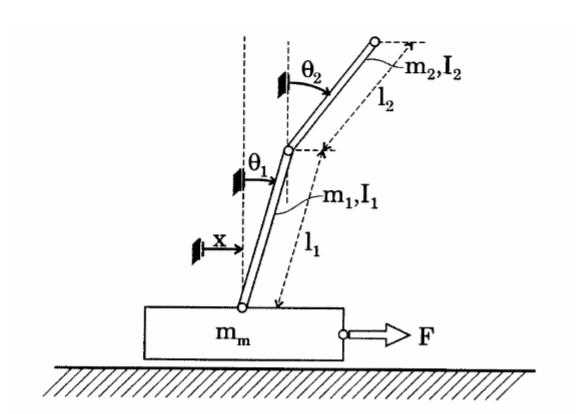
\includegraphics[width=15cm]{Modell_Doppelpendel}}
\caption{Mechanisches Modell eines stehenden Doppelpendels}
\end{figure}
\noindent

Da wir bei der Berechnung der Matrizen, welche für eine Zustandsraumdarstellung erfoderlich sind, einige Probleme hatten entschlossen wir uns sicherheitshalber mittels Euler-Lagrange-Formalismen auch die Bewegungsgleichungen neu aufzustellen und in MATLAB linearisieren zu lassen. Die Bewegungsgleichung erhalten wir mithilfe der Langrange Gleichung 2.Art.\\\\
$\dfrac{d}{dt}(\dfrac{\delta T}{\delta \dot{q_{i}}})-\dfrac{\delta T}{\delta q_{i}}+\dfrac{\delta V}{\delta q_{i}}=0$\\\\
Dafür werden die kinetische und die potentielle Energie benötigt. Die kinetische Energie setzt sich wiederum aus einem translatorischen und einem rotatorischen Anteil zusammen.\\\\
$ T=T_{trans}+T_{rot} $\\\\
Um den translatorischen Anteil zu berechnen werden die Geschwindigkeitsvektoren der Körper benötigt. \\\\
$ T_{trans}=\dfrac{1}{2} m \vec{v}^{2} $\\\\
$\vec{v}=Jv*\dot{q} $ \\\\
Die Jacobi-Matrix erhält man mit dem Befehl jacobian und besteht aus den partiellen Ableitungen der Ortsvektoren zu den Schwerpunkten nach den Minimalkoordinaten.
Der rotatorische Anteil wird mit Hilfe der Winkelgeschwindigkeitsvektoren der Stäbe und der Trägheitstensoren berechnet.\\\\
$ T_{rot}=\dfrac{1}{2} I_{s} \vec{\omega}^{2} $\\\\
Mit dem Befehl diag erfolgt die Festlegung der Trägheitstensoren als Diagonalmatrix, mit den Trägheitmomenten in der Diagonale.
Um die Energien in die Lagrange Gleichung 2.Art einsetzen zu können müssen sie partiell Abgeleitet werden (siehe Formel oben). Dies geschieht wiederum mit einer Jacobi-Matrix.
Die Linearisierung um die Gleichgewichtslage erhält man indem man alle Lagekoordinaten Null setzt. Der Befehl subs ersetzt dabei  $ \phi1 $,$ \phi2 $  , a und ihre Ableitungen mit 0.\\
	


\renewcommand{\thechapter}{}
\chapter{Implementierung in MATLAB}
\renewcommand{\thechapter}{3}
%
%%%%%%%%%%%%%%%%%%%%%%%%%%%%%%%%%%%%% *titel von section eventuell subsection wegen uebersicht*
%
MATLAB ist eine numerische Programmiersprache, welche für die schnelle Manipulation und Berechnung von Matrizen entwickelt wurde. Programmiert wird unter Matlab in einer proprietären Programmiersprache, die auf der jeweiligen Maschine interpretiert wird. Die Programmierung erfolgt hierbei textuell.

 \section{Variablendifinition und Modellbildung}
Bevor wir unser System simulieren lassen können, müssen wir unser mechanisches (Ersatz-)System in ein digitales Modell übersetzen. Dazu müssen dem Programm einige Parameter übergeben werden.\\
Zuerst werden Systemvariablen deklariert, sowie die Anzahl der Freiheitsgrade und Körper festgelegt. Außerdem wird ein Minimalkoordinatenvektor mit zugehörigen zeitlichen Ableitungen bestimmt.
\begin{lstlisting}
%Definition der Systemvariablen
syms l1 l2 phi_1 phi_2 phi_p1 phi_p2 phi_pp1 phi_pp2
syms a a_p a_pp mm m1 m2 g I_1 I_2 F xc

frg=3;                                     %Anzahl der Freiheitsgrade
n=3;                                       %Anzahl der Koerper

q=[a ; phi_1 ; phi_2];                     %Minimalkoordinaten
q_p=[a_p ; phi_p1 ; phi_p2];               %zeitliche Ableitungen
q_pp=[a_pp ; phi_pp1 ; phi_pp2];
\end{lstlisting}

\section{Simulation}
\section{Plot und Ausgabe}
\section{sourcecode}

\begin{lstlisting}
%---- Ermitteln der Bewegungsgleichungen
%     definieren der Systemvariablen
syms l1 l2 phi_1 phi_2 phi_p1 phi_p2 phi_pp1 phi_pp2
syms a a_p a_pp mm m1 m2 g I_1 I_2 F xc

frg=3;                                     %Anzahl der Freiheitsgrade
n=3;                                       %Anzahl der Koerper

q=[a ; phi_1 ; phi_2];                     %Minimalkoordinaten
q_p=[a_p ; phi_p1 ; phi_p2];               %zeitliche Ableitungen
q_pp=[a_pp ; phi_pp1 ; phi_pp2];

%---- Drehmatrix Stab 1
T_IK1 = [cos(phi_1) sin(phi_1) 0;
        -sin(phi_1) cos(phi_1) 0;
              0          0     1];
%---- Drehmatrix Stab 2
T_IK2 = [cos(phi_2) sin(phi_2) 0;
        -sin(phi_2) cos(phi_2) 0;
              0          0     1];

%---- Ortsvektoren
I_r_Sm = [a;0;0];
I_r_S1 = [a+l1/2*sin(phi_1) ; l1/2*cos(phi_1) ; 0];
I_r_Q2 = [a+l1*sin(phi_1) ; l1*cos(phi_1) ; 0];
K1_r_Q1S1 = [0; l1/2; 0];
K2_r_Q2S2 = [0; l2/2; 0];
I_r_S2 = I_r_Q2 + T_IK2 * K2_r_Q2S2;

%---- Traegheitstensoren in den koerperfesten Koordinatensystemen
K1_I_S1 = diag([0 0 I_1]);
K2_I_S2 = diag([0 0 I_2]);

%---- Winkelgeschwindigkeitsvektoren der Staebe
K_om1 = [0 ; 0 ; -phi_p1];
K_om2 = [0 ; 0 ; -phi_p2];

%---- JACOBI-Matrizen der Translation
J_Tm = jacobian(I_r_Sm, q);
J_T1 = jacobian(I_r_S1, q);
J_T2 = jacobian(I_r_S2, q);

%---- JACOBI-Matrizen der Rotation
J_R1 = jacobian(K_om1, q_p);
J_R2 = jacobian(K_om2, q_p);

%---- Geschwindigkeitsvektoren
I_v_Sm = J_Tm*q_p ;
I_v_S1 = J_T1*q_p ; 
I_v_S2 = J_T2*q_p ;

%---- kinetische Energie
T = 1/2*(mm*(I_v_Sm.'*I_v_Sm)+m1*(I_v_S1.'*I_v_S1)+m2*(I_v_S2.'*I_v_S2) ...%Translation
    +K_om1.'*K1_I_S1*K_om1+K_om2.'*K2_I_S2*K_om2);           %Rotation
T = simplify(T);                                             %Vereinfachung

%---- potentielle Energie
V=-(m1*I_r_S1.'+m2*I_r_S2.')*[0 ; -g ; 0];

%---- Ableitungen fuer LAGRANGEsche Gleichung 2. Art
dTdv = simplify(jacobian(T,q_p).');         %mit transponieren zu Spaltenvektor gemacht
dTdq = simplify(jacobian(T,q).');
dVdq = simplify(jacobian(V,q).');

%---- Elemente der Bewegungsgleichung M(q)*q_pp + f(q,q_p) = 0
disp('System-Massenmatrix M')
M = simplify(jacobian(dTdv,q_p))
disp('System-Vektorfunktion f')
f = simplify(jacobian(dTdv,q)*q_p+dVdq-dTdq-[F;0;0])

%==========================================================================
%---- Linearisierung um die Gleichgewichtslage:
%     phi_1 = 0, phi_2 = 0, a = 0

disp(' ')
disp('Elemente der linearisierten Bewegungsgleichung')
disp('System-Massenmatrix M0')
M0 = subs(M,{phi_1, phi_2, a},{0, 0, 0})
f0 = subs(f,{a, phi_1, phi_2, a_p, ...
    phi_p1, phi_p2},{0, 0, 0, 0, 0, 0});
disp('Auslenkungs-proportionaler Anteil')
Q = subs(jacobian(f,q),{a, phi_1, phi_2, a_p, ...
    phi_p1, phi_p2},{0, 0, 0, 0, 0, 0})
disp('Steifigkeitsmatrix K')
K = 1/2*(Q+Q.')
disp('Matrix der nichtkonservativen Kraefte')
N = 1/2*(Q-Q.')
disp('gesschw.-proportionaler Anteil')
P = subs(jacobian(f,q_p),{a, phi_1, phi_2, a_p, ...
    phi_p1, phi_p2},{0, 0, 0, 0, 0, 0})
disp('Daempfungsmatrix')
D = 1/2*(P+P.')
disp('gyroskopischer Anteil')
G = 1/2*(P-P.')

%==========================================================================
%----Erstellen und Simulieren der Zustandsraumdarstellung
syms x th1 th2 x_p th1_p th2_p
syms x_pp th1_pp th2_pp

y = [q.',q_p.'].';
y_p = [q_p.',x_pp , th1_pp , th2_pp].';

A = [zeros(3),eye(3);
    -M0^(-1)*Q, -M0^(-1)*P];
A = double(subs(A,{mm, m1, m2, l1, l2, g, I_1, I_2}, ...
    {0.2, 0.01, 0.01, 0.5, 0.7, 9.81, 2.0833e-04, 4.0833e-04}));
A(7,7) = 0;
A(7,1) = -1

B = [zeros(3,1);M0^(-1)*[1;0;0]];
B = double(subs(B,{mm, m1, m2, l1, l2, g, I_1, I_2}, ...
    {0.2, 0.01, 0.01, 0.5, 0.7, 9.81, 2.0833e-04, 4.0833e-04}));
B(7,1) = 0
Bxc = [0; 0; 0; 0; 0; 0; 1]

C = [1 0 0 0 0 0 0;
   0 1 0 0 0 0 0;
   0 0 1 0 0 0 0]

D = [0; 0; 0]


Q=eye(7);
r=1;

%----lqr Regelungsentwurf
k = lqr(A,B,Q,r)

%----neue Zustandsraumsystemmatrizen nach Parameterruekfuehrung
Ac = [(A-B*k)];
Bc = [Bxc];
Cc = [C];
Dc = [D];

states = {'x' 'th1' 'th2' 'x_p' 'th1_p' 'th2_p' 'in'};
inputs = {'F'};
outputs = {'x' 'th1' 'th2'};

sys_cl = ss(Ac,Bc,Cc,Dc,'statename',states,'inputname',inputs,'outputname',outputs);

%----definieren des Simulationszeitraums
t = 0:0.01:8;

%----definition des konstanten 0.2m offsets als Input
u =0.2*ones(size(t));

%----Simulation des erstellten Systems ueber gegebene Zeit mit bekanntem
%Input
[y,t,x]=lsim(sys_cl,u,t);


%----Drei einzelne Diagramme in einem Fenster
figure(1);
ax(1) = subplot(3,1,1);
    plot(ax(1),t,y(:,1),'b');
    title(ax(1),'cart position');     %Titel, Beschriftungen, Kommentare,
    ylim([-0.1,0.25]);                %andere Farben, andere skalierungen,
    grid on                           %da kann man sich noch frei austoben.
ax(2) = subplot(3,1,2);               %relativ einfach verstaendliche 
    plot(ax(2),t,y(:,2),'r');         %loesung. Ws nicht Laufzeit optimiert
    title(ax(2),'angle theta 1');
    grid on
ax(3) = subplot(3,1,3);
    plot(ax(3),t,y(:,3),'g');
    title(ax(3),'angle theta 2');
    grid on

%----Plotten der Ausgangsgroessen
% [AX,H1,H2] = plotyy(t,y(:,1),t,y(:,2),'plot');
% hold on
% line(t,y(:,3),'parent',AX(2),'color','g')
% hold off
% set(get(AX(1),'Ylabel'),'String','cart position (m)')
% set(get(AX(2),'Ylabel'),'String','pendulum angles (radians)')
% title('Step Response with LQR Control')

%----Berechnung der Eigenwerte
Eigenwerte = eig(Ac)
disp('Das System ist stabil, da der Realteil aller Eigenwerte negativ ist!')
\end{lstlisting}

\renewcommand{\thechapter}{}
\chapter{Implementierung in MalpeSim}
\renewcommand{\thechapter}{4}
Nachdem das vorherige Kapitel ausschließlich der Implementierung in MATLAB gewidment wurde, beschäftigt sich dieses Kapitel nun mit der Umsetzung in einer \textit{nicht klassischen}, blockorientierten, grafischen Programmierung in MapleSim. \\
Wie bereits erwähnt funktioniert die Programmierung in MapleSim grafisch. Es wird zuerst das Modell (in unserem Fall das geregelte mechanische Doppelpendel) im MapleSim GUI nachgebildet. Anschließend können Signale direkt an diesem Model abgegriffen und ins System rückgeführt werden.. Dadurch lassen sich selbst komplexe dynamische Systeme aus allen Bereichen der Natur- und Ingeneurswissenschaften vergleichsweise einfach modellieren.
\section{Modellbildung}
Da hier keine mathematischen Transformationen mehr nötig waren um das Doppelpendel in MapleSim modellieren zu können wurden direkt die Größen aus der Angabe verwendet. Die Materialparamter sind selbstverständlich die selben, wie die, die auch schon in den anderen Kapiteln verwendet wurden.

what what
\end{document}
